\documentclass[english,9pt,aspectraio=169]{beamer}
\usepackage{etex}
\usetheme{uzhneu-en-informal}
%\usepackage{uarial}
\usepackage[T1]{fontenc}
\usepackage[utf8]{inputenc}
\RequirePackage{graphicx,ae}
\usepackage{bm}
\usepackage{fancybox,amssymb,color}
\usepackage{pgfpages}
\usepackage{booktabs}
\usepackage{verbatim}
\usepackage{animate}
\usepackage{numprint}
\usepackage{vwcol} 
\usepackage{dsfont}
\usepackage{tikz}
\usepackage{amsmath,natbib}
\usepackage{mathbbol}
\usepackage{babel}
\usepackage{SweaveSlides}
\usepackage{multicol}
\usepackage{xcolor}


\usetheme{uzhneu-en-informal}
\DeclareMathOperator{\po}{Poisson}
\DeclareMathOperator{\G}{Gamma}
\DeclareMathOperator{\Be}{Beta}
\DeclareMathOperator{\logit}{logit}
\def\n{\mathop{\mathcal N}}

\definecolor{Gray}{RGB}{139,137,137}
\definecolor{darkred}{rgb}{0.8,0,0}
\definecolor{Green}{rgb}{0,0.8,0.3}
\definecolor{lightgreen}{rgb}{0,0.7,0.3}
\definecolor{Blue}{rgb}{0,0,1}
\def\myalert{\textcolor{darkred}}
\def\myref{\textcolor{Gray}}
\setbeamercovered{invisible}

\renewcommand{\baselinestretch}{1.2}
\beamertemplateballitem
\DeclareMathOperator{\cn}{cn} % Copy number
\DeclareMathOperator{\ccn}{ccn} % common copy number
\DeclareMathOperator{\p}{p} % common copy number
\DeclareMathOperator{\E}{E} % common copy number
\DeclareMathOperator{\given}{|} % common copy number
\def\given{\,|\,}
\def\na{\tt{NA}}
\def\nin{\noindent}
\pdfpageattr{/Group <</S /Transparency /I true /CS /DeviceRGB>>}
\def\eps{\varepsilon}

\renewcommand{\P}{\operatorname{\mathsf{Pr}}} % Wahrscheinlichkeitsmaß
\def\eps{\varepsilon}
\def\logit{\text{logit}}
%\newcommand{\E}{\mathsf{E}} % Erwartungswert
\newcommand{\Var}{\text{Var}} % Varianz
\newcommand{\Cov}{\text{Cov}} % Varianz
\newcommand{\NBin}{\text{NBin}}
\newcommand{\Po}{\text{Po}}
\newcommand{\N}{\mathsf{N}}

\newcommand{\hl}{\textcolor{red}}

\newcommand{\ball}[1]{\begin{pgfpicture}{-1ex}{-0.65ex}{1ex}{1ex}
\usebeamercolor[fg]{item projected}

{\pgftransformscale{1.75}\pgftext{\normalsize\pgfuseshading{bigsphere}}}
{\pgftransformshift{\pgfpoint{0pt}{0.5pt}}
\pgftext{\usebeamerfont*{item projected}{#1}}}
\end{pgfpicture}}%
\usepackage{multicol}
\newcommand{\ballsmall}[1]{\begin{pgfpicture}{-1ex}{-0.65ex}{.2ex}{.2ex}

{\pgftransformscale{1}\pgftext{\normalsize\pgfuseshading{bigsphere}}}
{\pgftransformshift{\pgfpoint{0pt}{0.5pt}}
\pgftext{\usebeamerfont*{item projected}{#1}}}
\end{pgfpicture}}%



\begin{document}

\fboxsep5pt

\frame{
\title[]{ \centering \Huge Kurs Bio144: \\
Datenanalyse in der Biologie}%\\[.3cm]
\author[Stefanie Muff, Owen L.\ Petchey]{\centering Stefanie Muff  \& Owen L.\ Petchey }
%\institute[]{Institute of Social and Preventive Medicine \\ Institute of Evolutionary Biology and Environmental Studies}
\date[]{Week 7: Model selection \\ 6./7. April 2017}


\maketitle
}


\frame{\frametitle{Overview (todo: check)}
\begin{itemize}
\item Model selection and model checking.\\[2mm]
\item Automatic model selection and its caveats.\\[2mm]
\item Selection criteria: AIC, BIC, Cp \\[2mm]
\item Model selection bias.\\[2mm]
\item Explanation v.s.\ prediction \\[2mm]
\item Relative importance of individual terms.\\[2mm]
\end{itemize}

 
}


\frame{\frametitle{Course material covered today}
\begin{itemize}
\item Stahel script chapters ...
\item Chapter 27.1 and 27.2 by Clayton and Hills ``Choice and Interpretation of Models'' (pdf provided)
\end{itemize}

\vspace{4mm}
\textcolor{blue}{\bf Optional reading:}
\begin{itemize}
\item Paper by \citet{freedman1983}
\item Check the Ellis book proposed by Owen
\end{itemize}
}

\frame[containsverbatim]{\frametitle{Recap of Last week}
\begin{itemize}
\item {\bf ANCOVA}
\item {\bf Linear alebra}
\end{itemize}
}

\frame{\frametitle{Developing a model}
So far, our regression models ``fell from heaven'': The model family and the terms in the model were almost always given.\\[4mm]

However, it is often \alert{not clear \emph{a priori}} which terms are relevant for a model. \\[2mm]

The two {\bf extreme situations} are\\[2mm]
\begin{enumerate}
\item \alert{It is clear/known} that $\bm{y}$ depends on a set of regressors $\bm{x}^{(1)}, \bm{x}^{(2)}, \ldots, \bm{x}^{(m)}$. \\[2mm]
\item The study has the aim \alert{to find connections} between the outcome $\bm{y}$ and the regressors. It is not known \emph{how} or \emph{if} each regressor influences $\bm{y}$.\\[2mm]
\end{enumerate}

The \alert{reality lies often in between}:\\
Interest centers around one predictor (e.g., a new medication), but the effect of other potential influence factors must be taken into account.
}

\frame{\frametitle{Why is finding a model so hard?}
Remember from week 1:\\[2mm]

\colorbox{lightgray}{\begin{minipage}{10cm}
Ein Modell ist eine Ann\"aherung an die Realit\"at. Das Ziel der Statistik und Datenanalyse ist es immer, dank Vereinfachungen der wahren Welt gewisse Zusammenh\"ange zu erkennen.
\end{minipage}}
\vspace{4mm}

Box (1979): \alert{``All models are wrong, but some are useful.''}\\[7mm]

$\rightarrow$ There is often not a ``right'' or a ``wrong'' model -- but there are more and less useful ones.\\[2mm]

$\rightarrow$ Finding a model with good properties is sometimes an art...\\[2mm]


}

\frame{
$\rightarrow$ Even among statisticians there is no real consensus about how (or if!) to do model selection:\\[2mm]


\includegraphics[width=10cm]{graphics/brewer_title.jpg}\\
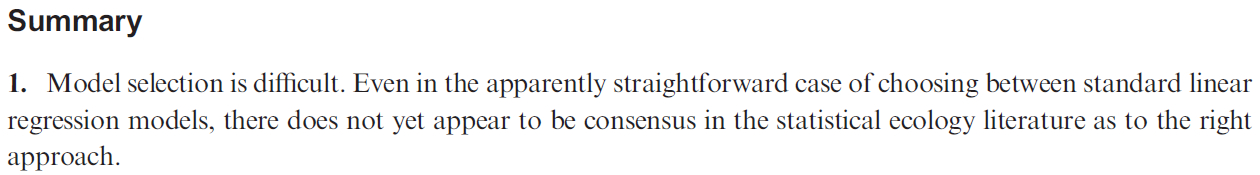
\includegraphics[width=10cm]{graphics/brewer.jpg}\\[2mm]

Note: The first sentence of a paper in \emph{Methods in Ecology and Evolution} from 2016 is: ``Model selection is difficult.''
}

\frame{\frametitle{Mercury example}
Let us look at the mercury example. The {\bf research question} was: \\
``Gibt es einen Zusammenhang zwischen Quecksilber(Hg)-Bodenwerten von Wohnh\"ausern und der Hg-Belastung im K\"orper (Urin, Haar) der Bewohner?''\\[2mm]
\begin{itemize}
\item \emph{Hg concentration in urine} is the {\bf response}.
\item \emph{Hg concentration in the soil} is the {\bf predictor of interest}.\\[5mm]
\end{itemize}

\alert{In addition}, the following variables were monitored for each person, because they might influence the mercury level in a person's body:\\[2mm]

\emph{Indicator if vegetables from garden are eaten; migration background; smoking status; number of amalgam fillings; age; number of monthly fish meals; indicator if fish was eaten in the last 3 days; mother; height; weight; BMI; sex; education level.}\\[2mm]

{\bf Thus: In total additional 13 variables!}
}


\frame{\frametitle{How many variables can I include in my model?}

{\bf Rule of thumb:}\\[1mm] 
\colorbox{lightgray}{\begin{minipage}{10cm}
Include no more than $n/10$ (10\% of $n$) variables into your linear regression model, where $n$ is the number of data points.
\end{minipage}}

~\\[2mm]
In the mercury example there are 156 individuals, so a {\bf maximum of 15 variables} should be included in the model.\\[2mm]

{\bf Remarks:}
\begin{itemize}
\item Categorical variables with $k$ levels already require $k-1$ dummy variables. For example, if `education level' has three categories, 2 variables are used up.\\[2mm]
\item Whenever possible, the model should {\bf not be blown up} unneccessarily. Even if there are many data points, the use of too many variables may lead to an {\bf overfitted} model
\end{itemize}
 

}



\frame{
In the mercury study, the following variables were included using \emph{a priori} knowledge:\\[4mm]

\begin{tabular}{llll}
Variable & Meaning & type & transformation\\
\hline
Hg$\_$urin & Hg conc.\ in urine (response) & continuous & $\log$\\ 
Hg$\_$soil & Hg conc.\ in the soil  & continuous & $\log$\\
vegetables & Eats vegetables from garden? & binary\\
migration & Migration background & binary \\
smoking & Smoking status & binary \\
amalgam & No.\ of amalgam fillings & count & $\sqrt{.}$ \\
age & Age of participant &  continuous\\ 
fish & Number of fish meals/month & count  & $\sqrt{.}$\\
last$\_$fish & Fish eaten in last 3 days? &   binary\\
mother & Mother or child?  & binary\\
\end{tabular}
\vspace{2mm}

}

% \frame{Ev list additional variables that were available in the mercury study. \\
% Examples: Height, weight, BMI, sex, the education level (3 categories), the duration of housing in the region (in months).\\[2mm]
% 
% say that no more than 10\% of the number of data points should be used in a model.}


\frame[containsverbatim]{Let us now fit the full model (including all covariates) in R:\\[2mm]


% latex table generated in R 3.3.2 by xtable 1.8-2 package
% Thu Dec 15 12:27:30 2016
\begin{table}[!h]
\centering
\begingroup\footnotesize
\begin{tabular}{rrrr}
  \hline
 & Coefficent & 95\%-confidence interval & $p$-value \\ 
  \hline
Intercept & -0.94 & from -1.10 to -0.79 & $<$ 0.0001 \\ 
  log10(Hg\_soil) & 0.03 & from -0.05 to 0.11 & 0.47 \\ 
  vegetables & 0.079 & from -0.03 to 0.19 & 0.15 \\ 
  migration & -0.048 & from -0.21 to 0.12 & 0.57 \\ 
  smoking & 0.23 & from 0.01 to 0.45 & 0.039 \\ 
  sqrt(amalgam) & 0.36 & from 0.27 to 0.45 & $<$ 0.0001 \\ 
  age & -0.0073 & from -0.02 to 0.01 & 0.32 \\ 
  mother & -0.04 & from -0.50 to 0.42 & 0.86 \\ 
  sqrt(fish) & 0.087 & from 0.03 to 0.14 & 0.003 \\ 
  last\_fish & 0.29 & from 0.13 to 0.44 & 0.0003 \\ 
   \hline
\end{tabular}
\endgroup
\end{table}
\vspace{3mm}
\begin{itemize}
\item We find $R^2=0.40$. Is this ``good''?\\[2mm]
\item Are there additional terms that might be important?\\[2mm]
\end{itemize}
}

\frame{
Remember from slides 7-10 of week 4 that the dependency of mercury in urine on age is different for mothers and children:

\begin{center}
\setkeys{Gin}{width=0.55\textwidth}
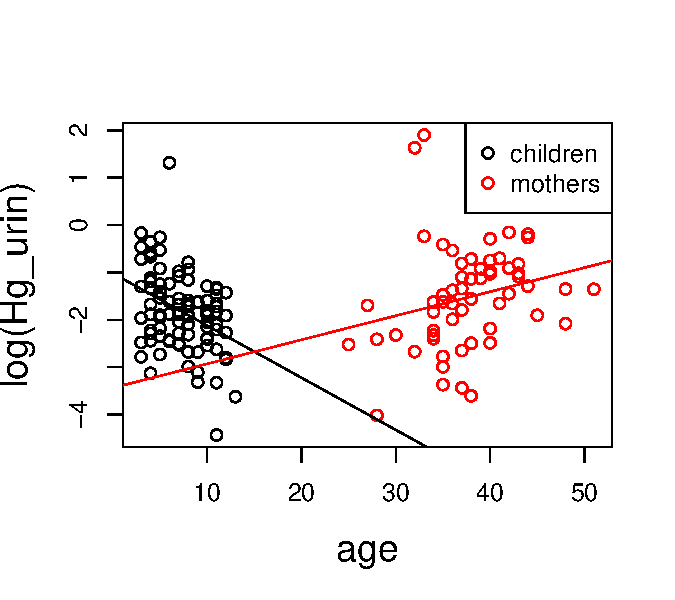
\includegraphics{Bio144_2017_week7-004}
\end{center}

$\rightarrow$ We need to include an interaction term \emph{mother}$\cdot$\emph{age}.
}

\frame[containsverbatim]{
Fitting the model again with the additional term:
% latex table generated in R 3.3.2 by xtable 1.8-2 package
% Thu Dec 15 12:27:30 2016
\begin{table}[!h]
\centering
\begingroup\footnotesize
\begin{tabular}{rrrr}
  \hline
 & Coefficent & 95\%-confidence interval & $p$-value \\ 
  \hline
Intercept & -0.68 & from -0.88 to -0.47 & $<$ 0.0001 \\ 
  log10(Hg\_soil) & 0.033 & from -0.05 to 0.11 & 0.42 \\ 
  vegetables & 0.07 & from -0.03 to 0.17 & 0.18 \\ 
  migration & -0.036 & from -0.19 to 0.12 & 0.65 \\ 
  smoking & 0.27 & from 0.06 to 0.48 & 0.012 \\ 
  sqrt(amalgam) & 0.33 & from 0.24 to 0.42 & $<$ 0.0001 \\ 
  age & -0.042 & from -0.06 to -0.02 & 0.0004 \\ 
  mother & -1.03 & from -1.70 to -0.35 & 0.003 \\ 
  sqrt(fish) & 0.079 & from 0.03 to 0.13 & 0.004 \\ 
  last\_fish & 0.30 & from 0.15 to 0.45 & $<$ 0.0001 \\ 
  age:mother & 0.055 & from 0.03 to 0.08 & 0.0002 \\ 
   \hline
\end{tabular}
\endgroup
\end{table}
\vspace{3mm}
\begin{itemize}
\item The $p$-value of the interaction is $<0.001$, thus very small.\\[2mm]
\item $R^2$ has now clearly increased to $0.45$.\\[2mm]
\end{itemize}

$\rightarrow$ The interaction term apparently improved the model.
}

\frame[containsverbatim]{
A model checking step (always needed, but we did it already in weeks 4)
\setkeys{Gin}{width=0.8\textwidth}
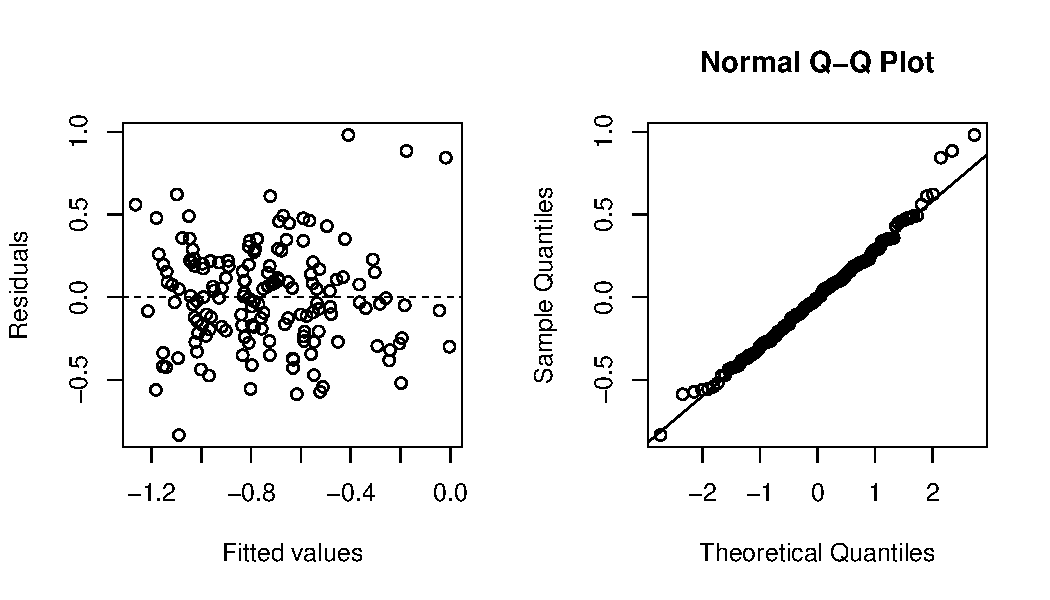
\includegraphics{Bio144_2017_week7-modelChecksHg}
\vspace{2mm}

This looks ok, no need to improve the model from this point of view.
}

\frame{
Even if the model checking step revealed no violations of the assumptions (the model seems to be fine), we usually want to know:\\[2mm]

\begin{itemize}
\item Which of the terms are \alert{important/relevant}?\\[2mm]
\item Are there \alert{additional terms} that might be important?\\[2mm]
\item Would it be possible to further \alert{``improve'' the model}?\\[3mm]
\end{itemize}
\vspace{3mm}

Often, the desire is to find a model that is in some sense ``optimal'' or ``best''.  
}


\frame{\frametitle{Is importance reflected by $p$-values?}
A widely used practice to determine the ``importance'' of a term is to look at the $p$ value from the $t$-test and check if it falls below a certain threshold (usually $p<0.05$). \\[4mm]

{\bf However, there are a few problems with this approach:}\\[2mm]

\colorbox{lightgray}{\begin{minipage}{10cm}
\begin{itemize}
\item When carrying out the $t$-tests with $H_0: \beta_j=0$ for all variables , one runs into a \alert{multiple testing problem}.\\
{(\scriptsize Remember the ANOVA lecture, week 5, slide 25).}\\[2mm]
\item The respective tests depend crucially on the correctness of the \alert{normality assumption}.\\[2mm]
\item Covariates are sometimes \alert{collinear}, which leads to more uncertainty in the estimation of the respective regression parameters, and thus to larger $p$-values.\\[2mm]
\item {\bf A small $p$-value does not necessarily mean that a term is (biologically, medically) important -- and vice versa!}
\end{itemize}
\end{minipage}}
}

\frame{
For all these reasons, we {\bf strongly disagree} with the remark in Stahel's script 5.2, second part in paragraph d.\\[4mm]

The first part is ok:\\[2mm]

\includegraphics[width=10cm]{graphics/52d_1.pdf}\\[2mm]

But we disagree with this:\\[2mm]

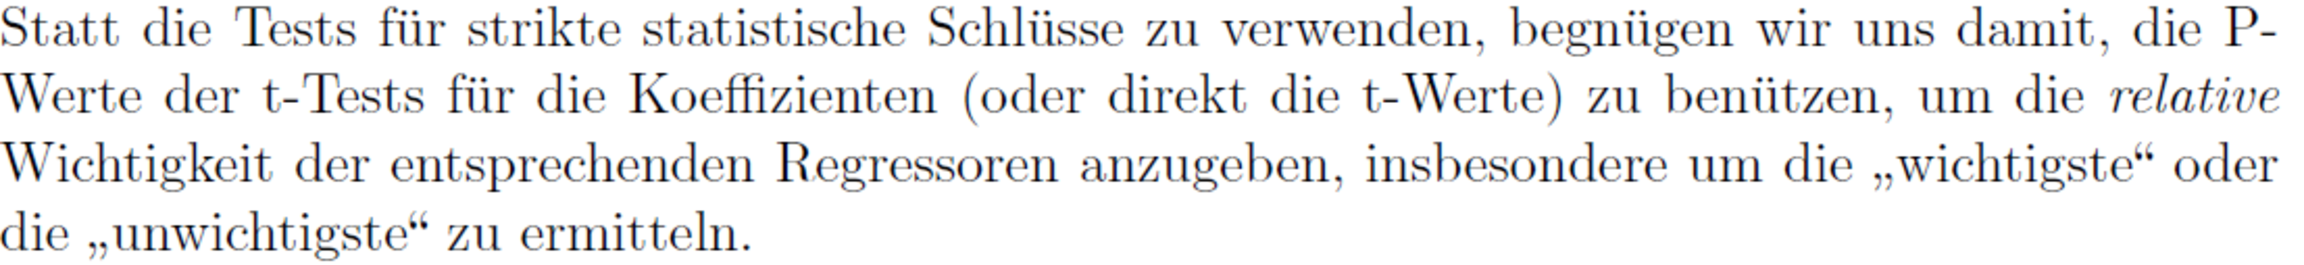
\includegraphics[width=10cm]{graphics/52d_2.pdf}
}


\frame{\frametitle{Automatic model selection procedures}
It would be very convenient if there were {\bf objective} or even {\bf automatic} procedures to select the ``best'' model. Wouldn't it?\\[2mm]

In fact, such procedures have been proposed in the past. For example:\\[4mm]
\begin{itemize}
\item \alert{Forward selection:}\\
Start with a large/full model. In each step, remove the variable with the largest $p$-value. Do this until only variables with low $p$-values remain in the model.\\[4mm]
\item \alert{Backward selection:}\\
Start with an empty model. In each step, add the predictor with the highest importance (lowest $p$-value). Do this until none of the missing coefficients has a low $p$-value when adding it.\\[2mm]
\end{itemize}


}

\frame{\frametitle{Important note}
\colorbox{lightgray}{\begin{minipage}{10cm}
{\bf However: Automatic model selection procedures may lead to biased parameter estimates and wrong conclusions!}
\end{minipage}}
{\scriptsize See, e.g., \citet{freedman1983, copas1983}.}
\vspace{4mm}

Please note that {\bf we strongly discourage the use of automated model selection procedures}. So please ignore large parts of chapter 5.3 in the Stahel script!! \\[2mm]

Or read it to see how you should {\bf not} do it.
}

\frame{\frametitle{More modern ways to do model selection}

\underline{Remember:} $R^2$ is not suitable for model selection, because it \emph{always} increases (improves) when a new variable is included.\\[4mm] 

In 2002, Burnham and Anderson suggested the use of so-called \alert{information-criteria} for model selection. \\[4mm]

The idea is to find a \alert{balance between}\\[4mm]

\begin{center}
{\bf Good model fit} $\quad\leftrightarrow\quad$ {\bf Low model complexit}
\end{center}

~\\[4mm]
$\rightarrow$ Penalize models with more parameters.
}

\frame{
The most prominent criterion is the \alert{AIC (Akaike Information Criterion)}, which measures the \alert{quality of a model}.\\[2mm]

\colorbox{lightgray}{\begin{minipage}{10cm}
The AIC of a model with likelihood $L$ and $p$ parameters is given as
\begin{equation*}
AIC = -2\log(L) + 2p
\end{equation*}
\end{minipage}}

~\\[4mm]
{\bf Important: The \underline{lower} the AIC, the \underline{better} the model!}\\[6mm]

The AIC is a \alert{compromise} between
\begin{itemize}
\item a high likelihood $L$ (good model fit) 
\item few model parameters $p$ (low complexity)
\end{itemize}

}

\frame[containsverbatim]{\frametitle{Example of AIC use}
Remember that we first fitted the mercury example {\bf without} (\texttt{r.lm}) and {\bf with} (\texttt{r.lm2}) the interaction $mother\cdot age$. The model improvement is also confirmed by the {\bf reduction in AIC}:\\[6mm]

\begin{Schunk}
\begin{Sinput}
> AIC(r.lm)
\end{Sinput}
\begin{Soutput}
[1] 107.4609
\end{Soutput}
\begin{Sinput}
> AIC(r.lm2)
\end{Sinput}
\begin{Soutput}
[1] 94.48769
\end{Soutput}
\end{Schunk}
~\\[4mm]
\underline{Interpretation:} The AIC of the model with interaction is clearly lower, thus the model with interaction is to be preferred.\\[4mm]

}

\frame[containsverbatim]{
We can further play around with AIC and, for instance, fit a model withouth the binary \emph{migration} variable:\\[4mm]

\begin{Schunk}
\begin{Sinput}
> r.lm3 <- lm(log10(Hg_urin) ~ log10(Hg_soil) + vegetables  + smoking + 
+              sqrt(amalgam) + age * mother + sqrt(fish) + last_fish,d.hg)
> AIC(r.lm3)
\end{Sinput}
\begin{Soutput}
[1] 92.70363
\end{Soutput}
\end{Schunk}

~\\[4mm]
\underline{Interpretation:} We observe a further reduction of AIC. \\[4mm]

This success brings us to another idea:\\[2mm]
\colorbox{lightgray}{\begin{minipage}{10cm}
{\bf Could we do model selection simply by minimizing the AIC?}\\
Without actually ``thinking''?
\end{minipage}}
}

\frame{
\begin{itemize}
\item AIC for `all subsets selection'\\
For $m$ variables there are $2^m$ possible models. Fit all models and take the ``best'' one (lowest AIC or BIC).\\[2mm]
\item Caveates and recommended practice
\end{itemize}
}

\frame{\frametitle{BIC, the brother of AIC}
Definition and connection to AIC.
}


\frame{\frametitle{Model selection bias}
\citet{freedman1983} example
}



\frame[containsverbatim]{\frametitle{The bodyfat example}
Say that here we aim at prediction, not at explanation and that these are different situations in terms of model selection.

}



\frame{\frametitle{Summary}

}
\frame{References:
\bibliographystyle{Chicago}
\bibliography{refs}
}



\end{document}
